% Use ACM Article class. The SIGCOMM '27 template ships with [sigconf,anon,review].
% `anon` and `review` are dropped: this final course copy names its authors and omits line numbers.
% For a double-blind review version, restore: \documentclass[sigconf,anon,review]{acmart}
\documentclass[sigconf]{acmart}

% Package for balancing columns on final page
\usepackage{balance}
\usepackage{booktabs}
\usepackage{multirow}
\usepackage{algorithm}
\usepackage{algpseudocode}
\usepackage{xspace}

% Copyright and Conference settings -- mostly supressed for submission
\renewcommand\footnotetextcopyrightpermission[1]{}
\settopmatter{printacmref=false, printccs=false, printfolios=true}
\acmConference{ACM SIGCOMM 2027 Conference}{August 8--12, 2027}{Bangkok, Thailand}

\newcommand{\cmabp}{CMAB+\xspace}
\newcommand{\oldcmab}{old CMAB\xspace}
\newcommand{\That}{\hat{T}}
\newcommand{\kbps}{\,kbps\xspace}
\setlength{\emergencystretch}{1.5em}

% Title Block
\title{Repairing Forced-Rung Collapse in Contextual-Bandit Live Streaming over Starlink-Like Links}
\subtitle{CS G525 Advanced Computer Networks, Track A7: reproduction, transport extension, and CMAB+}

% Author Block
\author{Pratham Shah}
\affiliation{%
  \position{2026H1030063P}
  \institution{BITS Pilani}
  \city{Pilani}
  \country{India}}
\author{Vidhu Kant Sharma}
\affiliation{%
  \position{2026H1030053P}
  \institution{BITS Pilani}
  \city{Pilani}
  \country{India}}
\author{Ved Pahune}
\affiliation{%
  \position{2026H1030056P}
  \institution{BITS Pilani}
  \city{Pilani}
  \country{India}}
\author{Yash Sinha}
\affiliation{%
  \position{Course Tutor}
  \institution{BITS Pilani}
  \city{Pilani}
  \country{India}}
\renewcommand{\shortauthors}{Shah et al.}

\begin{document}

%% BEGIN BODY
\begin{abstract}
Starlink reassigns satellites to user terminals every 15\,s, and each reassignment raises latency and loss. Zhao and Pan (MMSys '24) built a contextual-bandit bitrate controller (CMAB) for low-latency DASH live streaming that restarts its learning at each of these handovers. We reproduced their emulation and repeated it under BBR congestion control. A first BBR run that looked like a transport failure had used the wrong traffic shaper, and tracing it exposed a flaw in the controller itself: after every handover it requests the top 6000\kbps rung for seven decisions without checking throughput, so on slower links the player stalls continuously. We keep the bandit and add five rules, which we call CMAB+, that cap each request at measured throughput and hold a low rung after a stall. Across 450 emulated sessions, CMAB+ matches the original controller on the artifact's 100\,Mbit/s shaper. On a 4\,Mbit/s bottleneck it cuts rebuffering from 62--82\% to 0\% at every latency target. On a replayed Starlink inter-satellite-link trace it cuts rebuffering by 71--86\%, though the dash.js baseline L2A-LL still rebuffers less there. Bandit exploration in live streaming should be bounded by what the link has delivered.
\end{abstract}

\maketitle

\section{Introduction}

Live video has little room to hide network trouble. A video-on-demand (VoD) player can hold tens of seconds of media; a low-latency live player aiming at 3\,s behind the live edge holds one or two 2\,s segments. Starlink adds a periodic disturbance to that budget. Satellite-to-ground scheduling is reconfigured every 15\,s, at seconds 12, 27, 42 and 57 of each minute, and round-trip time (RTT) and loss jump at those instants~\cite{tanveer2023constellations,pan2023measuring}.

Zhao and Pan~\cite{zhao2024mmsys} measured this pattern and proposed an adaptive bitrate (ABR) controller for the dash.js player~\cite{dashjs} for Dynamic Adaptive Streaming over HTTP (DASH) that knows the slot boundaries. It treats each rung of the bitrate ladder as an arm of a contextual bandit, learns with Linear Thompson Sampling (LinTS)~\cite{agrawal2013thompson}, and discards its history at every boundary. They evaluated it in a Docker emulator and on a real dish, against the three low-latency ABRs shipped with dash.js: Dynamic~\cite{spiteri2019dynamic}, Learn2Adapt-LowLatency (L2A-LL)~\cite{karagkioules2020l2a} and LoL+~\cite{bentaleb2022lolp}. We call their controller \emph{\oldcmab} below.

This report covers a semester project in three phases. Review~I reproduced the paper's emulation results under the artifact's default TCP, CUBIC~\cite{ha2008cubic}. Review~II asked whether the transport matters and repeated the matrix under BBR~\cite{cardwell2016bbr}. The first BBR run showed CMAB far off its target; tracing that result back led to a testbed mistake and then to a design flaw in \oldcmab. Review~III fixed that flaw. The contributions are:

\begin{itemize}
\item A reproduction of the paper's emulation campaign (160 sessions of 300\,s) and a matching BBR campaign. Under the paper's clock shaper, CMAB at a 3\,s target behaves similarly under both transports (3.19\,s and 3.29\,s, no rebuffering). We could not reproduce one claim: the paper reports every ABR missing a 3\,s target by at least 1.5\,s, and in our CUBIC reproduction none missed by more than 0.19\,s (Section~\ref{sec:repro}).
\item A testbed lesson. The first BBR result came from running the trace shaper instead of the clock shaper; separately, the trace shaper broke on container restart. We separate the three resulting datasets and report which claims each one supports (Section~\ref{sec:bbr}).
\item A diagnosis of \emph{forced-rung collapse}: \oldcmab requests the top rung during the first $|A|-1$ decisions of every slot without checking throughput, so a link slower than that rung stalls continuously (Section~\ref{sec:diagnosis}).
\item \cmabp, which keeps the paper's LinTS learner, reward and catch-up policy and adds five rules. We report the designs we rejected on the way (Section~\ref{sec:design}).
\item An evaluation over 450 sessions on three shapers and two transports, with 95\% confidence intervals: no regression on the paper's clock shaper, a fix for collapse at 4\,Mbit/s at every target, and lower rebuffering on a Starlink trace. L2A-LL remains the better choice where rebuffering matters most (Section~\ref{sec:eval}).
\end{itemize}

All of this is emulation. We had no Starlink dish, so the trace results replay a recorded latency trace through \texttt{tc}. \cmabp is a systems repair of one implementation, not a new bandit algorithm.

\section{Background}
\label{sec:background}

\paragraph{Starlink handovers.} Tanveer et al.~\cite{tanveer2023constellations} showed that Starlink reallocates user terminals to satellites on a global 15\,s schedule. Pan et al.~\cite{pan2023measuring} and Zhao and Pan~\cite{zhao2024mmsys} measured latency spikes at seconds 12, 27, 42 and 57 from installations in North America and the Seychelles, where traffic crosses laser inter-satellite links (ISLs) to reach a ground station. The paper reports a median RTT to the gateway of 42.8\,ms without ISLs and 109.0\,ms with them. Their measurements are published as the LENS dataset~\cite{zhao2024lens}.

\paragraph{Low-latency DASH.} A DASH player~\cite{sodagar2011dash} downloads fixed-duration segments, each available at several bitrates (the \emph{ladder}). The artifact uses an eight-rung ladder of 300, 450, 900, 1200, 1500, 4900, 5100 and 6000\kbps with 2\,s segments, served live by livesim2~\cite{livesim2}. Live latency is the distance between the playback position and the live edge. When it drifts from the target, a catch-up controller changes playback speed. dash.js ships three low-latency ABRs: Dynamic switches between a throughput rule and BOLA~\cite{spiteri2020bola}; L2A-LL uses online convex optimization; LoL+ uses a self-organizing map with its own playback-speed control. O'Hanlon and Aslam~\cite{ohanlon2023latency} compared these three on terrestrial traces.

\paragraph{CMAB in MMSys '24.} Before each segment, \oldcmab observes a context of measured network latency, playback speed and estimated throughput, and picks an arm with LinTS from MABWiser~\cite{strong2021mabwiser}, run in the browser through Pyodide~\cite{pyodide}. The reward multiplies the ITU-T P.1203 O.46 score~\cite{itu2017p1203} by the ratio of target to measured latency and by a bitrate ratio, then subtracts the share of the session's rebuffering time spent at the chosen bitrate. History only covers the current 15\,s slot. The implementation adds two details that matter here. During the first $|A|-1$ decisions of each slot it selects the top rung instead of calling LinTS, and it applies every switch at dash.js \texttt{STRONG} priority, which overrides the throughput rule. Neither detail is part of the LinTS formulation in the paper.

\section{Review I: reproducing the emulation}
\label{sec:repro}

\paragraph{Setup.} We ran the authors' artifact~\cite{zhao2024artifact} (commit \texttt{dc120de}) on one Google Cloud \texttt{e2-standard-4} virtual machine (VM; 4 vCPU, 16\,GB) in \texttt{asia-south1-c}. Docker Compose starts livesim2, an nginx front end that also hosts the traffic shaper, a stats server with MongoDB, and a Selenium-driven Chromium running the modified dash.js 4.7.1. The default \emph{clock} shaper (\texttt{tc.py}) applies a token-bucket filter and netem on nginx's egress: 100\,Mbit/s, 40\,ms delay and 0.1\% loss, switched to 50\,Mbit/s, 100\,ms and 1\% loss during each handover second. The matrix is the paper's: four ABRs, targets of 3, 4, 5 and 6\,s, ten rounds of 300\,s each, 160 sessions in total, all under CUBIC.

\paragraph{Results.} Table~\ref{tab:review12} gives the 3\,s row; Appendix~\ref{app:review12} has all targets. The qualitative picture matches the paper. All four ABRs track the target, CMAB sits a little above the others (3.19\,s against 3.00--3.08\,s at 3\,s), and L2A-LL plays the top rung throughout. One prediction failed. The paper says that at a 3\,s target every algorithm misses by at least 1.5\,s. In our runs the worst miss at 3\,s was 0.19\,s. We do not know the cause. Our metric drops the first 20\% of each session (Section~\ref{sec:method}), which removes start-up, and the paper's own metric pipeline may differ.

Under our metric, every cell except one has a mean rebuffer ratio of 0.00\%. The exception is one CMAB round at the 5\,s target with 13.38\,s mean latency and 25.24\% rebuffering; the other nine rounds sat at 5.21--5.38\,s with none. That single round lifts the cell mean to 6.05\,s and 2.52\%. We kept it in every aggregate and report it here instead of dropping it.

\begin{table}[t]
\caption{Review I and II at a 3\,s target: mean of 10 sessions. D1 is the Review I reproduction, D3 the BBR rerun on the clock shaper, D2 the first BBR run on the trace shaper. Latency in s, rebuffer ratio in \%, bitrate in kbps.}
\label{tab:review12}
\small
\begin{tabular}{@{}lrrrrrr@{}}
\toprule
 & \multicolumn{2}{c}{D1: CUBIC, clock} & \multicolumn{2}{c}{D3: BBR, clock} & \multicolumn{2}{c}{D2: BBR, trace} \\
\cmidrule(lr){2-3}\cmidrule(lr){4-5}\cmidrule(l){6-7}
ABR & Lat. & kbps & Lat. & kbps & Lat./Reb. & kbps \\
\midrule
Dynamic & 3.00 & 5909 & 3.12 & 5123 & 4.13 / 1.10 & 619 \\
L2A-LL  & 3.00 & 6000 & 3.11 & 6000 & 3.81 / 0.59 & 359 \\
LoL+    & 3.08 & 4938 & 3.14 & 5454 & 4.64 / 5.40 & 861 \\
CMAB    & 3.19 & 4955 & 3.29 & 5223 & 7.19 / 28.32 & 5795 \\
\bottomrule
\end{tabular}

\smallskip
\footnotesize Rebuffer ratio is 0.00\% in every D1 and D3 cell shown except LoL+ under D3 (0.01\%).
\end{table}

\section{Review II: BBR and a shaper confound}
\label{sec:bbr}

The extension asked whether a handover is mainly an ABR problem or a transport problem. BBR (Bottleneck Bandwidth and Round-trip propagation time) models bottleneck bandwidth and minimum RTT and paces its sending rate instead of backing off on every loss~\cite{cardwell2016bbr}, so it could recover from a lossy handover second faster than CUBIC. We switched the nginx container's congestion control to BBR with \texttt{sysctl}, kept the ABRs and batch file unchanged, and reran the 160-session matrix.

\paragraph{The first run.} The first complete BBR matrix (session prefix \texttt{1010-0432}) put CMAB at 7.19\,s latency and 28.32\% rebuffering at a 3\,s target, while Dynamic dropped to 619\kbps and kept latency at 4.13\,s (Table~\ref{tab:review12}, D2). Before attributing this to BBR, we ran a small validation on the patched stack under CUBIC. CMAB failed there too: our Review~II notes record about 16.6\,s latency, 86\% rebuffering and all 28 logged decisions on the top arm. A transport effect could not explain a CUBIC failure, so we audited the testbed.

\paragraph{Root causes.} We found two faults. First, the run selected the trace shaper (\texttt{SHAPER=trace}). It replays a one-hour Starlink ISL latency trace with a median RTT of about 130\,ms and 100\% loss at handover rows. Review~I had used the clock shaper, and the two shapers are different experiments. Second, the batch runner restarts nginx before every session. A Docker restart keeps the network namespace and its old qdiscs, and the trace shaper's initialization only added classes, so it crashed on restart and could leave the link stuck in a 100\%-loss state. This second fault is a reliability problem; the first explains the D2 numbers, since the corrected trace shaper in Review~III gave \oldcmab almost the same result under BBR (7.16\,s and 28.98\% at 3\,s, Section~\ref{sec:trace}). We rewrote the initialization to delete and rebuild the HTB root, verified the shaper mode inside the container before each batch, and reran the full matrix with the clock shaper (prefix \texttt{1017-0606}).

\paragraph{The clock-shaper comparison.} Under the clock shaper, BBR changes little (Table~\ref{tab:review12}, D3; Figure~\ref{fig:review2}). CMAB at 3\,s moves from 3.19 to 3.29\,s with no rebuffering, and its bitrate rises from 4955 to 5223\kbps. The other ABRs stay within 0.12\,s of their CUBIC latency. On this path the transport has a small effect.

\begin{figure}[t]
\centering
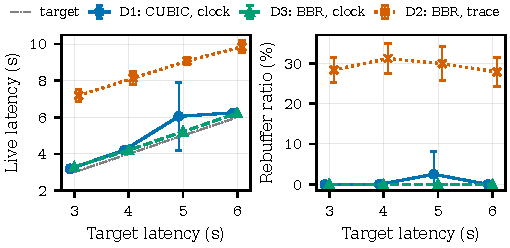
\includegraphics[width=\columnwidth]{figures/review2-cmab}
\Description{Line plots of CMAB latency and rebuffer ratio against latency target for datasets D1, D3 and D2.}
\caption{CMAB under the three Review I/II datasets, mean of 10 sessions with 95\% $t$ intervals. Under the clock shaper, CUBIC (D1) and BBR (D3) both track the target; the D1 spike at 5\,s is one outlier round. The large latency and rebuffering of D2 come from the trace shaper.}
\label{fig:review2}
\end{figure}

The labels are: D1 is CUBIC on the clock shaper, D2 BBR on the trace shaper and D3 BBR on the clock shaper. D2 supports no transport claim. It did show one controller effect: on the same trace, Dynamic adapted down to 619\kbps and survived, while CMAB kept requesting about 5800\kbps. That difference pointed at the controller.

\section{Diagnosing forced-rung collapse}
\label{sec:diagnosis}

Reading \texttt{CMABAbrController.js} and \texttt{CMABRule.js} gave a direct explanation. After each slot boundary, while fewer than $|A|-1=7$ decisions have been made in the slot, the controller returns the top arm without consulting LinTS or the throughput estimate. The switch is issued at \texttt{STRONG} priority, so dash.js's throughput rule cannot lower it.

Two pieces of arithmetic show why this matters. A slot is 15\,s and a segment is 2\,s, so a player keeping pace makes about seven or eight decisions per slot, and the forced window covers almost all of them. And one 6000\kbps segment carries 12\,Mbit, which takes at least 3\,s to fetch over a 4\,Mbit/s link. Every forced decision therefore downloads slower than it plays, the buffer drains, and a stalled player makes even fewer decisions per slot, so LinTS may never get a turn before the next reset. We call this \emph{forced-rung collapse}.

On the artifact's 100\,Mbit/s clock shaper the top rung fits and the forced window is harmless, which is why Review~I and the D3 rerun look healthy. Collapse appears when delivered throughput falls below the top rung, as on the trace shaper, where RTT and handover loss hold TCP well below the 50\,Mbit/s ceiling. Figure~\ref{fig:timeline} shows it on a fixed 4\,Mbit/s link. Old CMAB requests 6000\kbps for the whole minute and its buffer sits at the 0.05\,s floor between short refills. \cmabp, described next, holds the 1500\kbps rung and keeps the buffer between about 0.5 and 2.5\,s.

\begin{figure}[t]
\centering
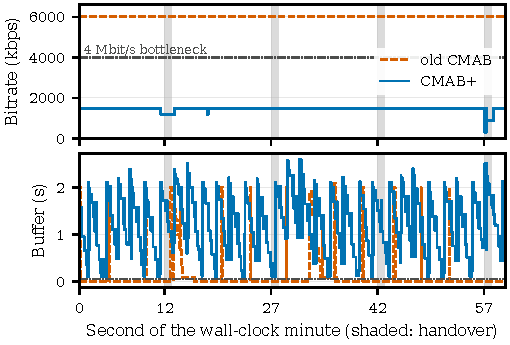
\includegraphics[width=\columnwidth]{figures/timeline-4mbit}
\Description{Two stacked time series over one minute: requested bitrate and buffer level for old CMAB and CMAB+ on a 4 Mbit/s link.}
\caption{One minute of one session per player on a 4\,Mbit/s clock shaper (CUBIC, 3\,s target, round 0; the first full minute after 120\,s of playback, handover seconds shaded). Top: requested bitrate. Bottom: playback buffer, with the 0.05\,s rebuffer threshold dashed. Old CMAB stays on the 6000\kbps rung and its buffer keeps hitting the floor.}
\label{fig:timeline}
\end{figure}

\section{CMAB+ design}
\label{sec:design}

\cmabp keeps LinTS, the context vector, the reward, the 15\,s slot reset and the catch-up policy. It changes what happens around the bandit's choice. Let $r_i$ be the bitrate of arm $i$, $\That$ the throughput estimate from dash.js \texttt{getSafeAverageThroughput} (already multiplied by its 0.9 safety factor), $q$ the quality currently playing, and $i^\star=\max\{i: r_i\le\That\}$ the highest feasible arm ($i^\star=0$ if $\That$ is missing). The five rules are:

\begin{enumerate}
\item \emph{Feasible probe.} In the first $|A|-1$ decisions of a slot, request $i^\star$ instead of the top arm. LinTS is skipped in this window, as in \oldcmab.
\item \emph{Throughput clamp.} After the window, the LinTS arm is capped at $i^\star$.
\item \emph{Throughput-triggered step-down.} If $r_q>\That$, the arm cannot rise on this decision and is at most $q-1$. Otherwise the clamped suggestion stands, including a jump up to $i^\star$.
\item \emph{Switch priority.} An upward switch that rule~2 reduced uses \texttt{DEFAULT} priority, so other dash.js rules may veto it. All other switches keep \texttt{STRONG}.
\item \emph{Stall guard.} When a real quality is playing and the buffer is at or below 0.05\,s, the arm cannot rise and is capped at the highest rung that fits the worst of the last eight segment throughputs, scaled by the same 0.9 safety factor. The guard turns off after 12 consecutive decisions with at least 1\,s of buffer.
\end{enumerate}

\noindent Algorithm~\ref{alg:cmabplus} gives one decision. The flag \texttt{cmabHardened=true} enables the rules for \texttt{abrCMAB} only; the other ABRs are unchanged. The code is in \texttt{cmabPlusPolicy.js}, with unit tests, in the project repository~\cite{cmabplus}.

\begin{algorithm}[t]
\caption{One CMAB+ decision}
\label{alg:cmabplus}
\small
\begin{algorithmic}[1]
\Require ladder $r_0<\dots<r_{|A|-1}$, estimate $\That$, playing quality $q$, buffer $b$, decisions $n$ in this slot, guard state $g$
\State $i^\star \gets \max\{i : r_i \le \That\}$, or $0$ if $\That$ is missing
\If{$n < |A|-1$} $s \gets i^\star$ \Comment{rule 1; old CMAB sets $s \gets |A|-1$}
\Else\ $s \gets \textsc{LinTS.select}()$
\EndIf
\State $a \gets \min(s, i^\star)$;\ \ $clamped \gets (a \ne s)$ \Comment{rule 2}
\If{$q \ge 0$ \textbf{and} $r_q > \That$} $a \gets \min(a, \max(0, q-1))$ \Comment{rule 3}
\EndIf
\State $g \gets \textsc{UpdateGuard}(g, b, q)$ \Comment{on if $b\le 0.05$\,s; off after 12 decisions with $b\ge 1$\,s}
\If{$g.\mathit{active}$}
  \State $w \gets 0.9 \times \min$ of the last 8 segment throughputs
  \State $a \gets \min(a, q, \max\{i : r_i \le w\})$ \Comment{rule 5}
\EndIf
\State $p \gets \texttt{DEFAULT}$ \textbf{if} $clamped$ \textbf{and} $a>q$ \textbf{else} \texttt{STRONG} \Comment{rule 4}
\State request arm $a$ at priority $p$; record reward; $n \gets n+1$
\end{algorithmic}
\end{algorithm}

\paragraph{Designs we rejected.} We reached these rules through eight trials: seven full or partial matrices on the clock shaper and an eighth on the capacity shaper (Table~\ref{tab:trials}). Removing the forced window without a replacement (trial~1) left CMAB at 900\kbps at every target, so the bandit needs a probe. A feasible probe and clamp alone (trial~2) recovered bitrate but missed a 3\,s target by 2\,s under BBR. Trials 3 to 7 tried live latency as the step-down trigger. Stepping down whenever latency exceeded the target walked the ladder to 300\kbps, because a healthy player runs slightly above its target. A 1\,s margin looked fine under BBR but under CUBIC sat on the margin line (4.02\,s at a 3\,s target) and cut bitrate to 3009\kbps on a link that carried 4955\kbps for \oldcmab. Trial~8 replaced latency with throughput as the trigger and is the core of \cmabp. Rule~5 came last, from trace runs: before it, CMAB+ still rebuffered 31--35\% on the trace under CUBIC. Variants of the guard that kept a spare rung below $\That$ or forced the bottom rung were flat or worse and were dropped.

\begin{table}[t]
\caption{Design ledger: CMAB+ trials at a 3\,s target. Lat./Reb./kbps are mean live latency (s), rebuffer (\%) and bitrate (kbps). Old CMAB on the same clock shaper: 3.19/0/4955 (CUBIC) and 3.29/0/5223 (BBR).}
\label{tab:trials}
\footnotesize
\begin{tabular}{@{}clll@{}}
\toprule
\# & Change & Run & Result at 3\,s \\
\midrule
1 & no top-rung probe & BBR clock & 900\kbps at every target \\
2 & feasible probe + clamp & BBR clock & 4.99 s / 1.0\% / 5200--5400 \\
3 & step down if late & BBR (partial) & 3.17 s / 0\% / 300 \\
4 & step down if $>$1\,s late & BBR clock & 3.32 s / 0\% / 4894 \\
4 & same & CUBIC (partial) & 3.98 s / 0\% / 3035 \\
5 & + one-rung climb & CUBIC clock & 3.85 s / 0.04\% / 2626 \\
6 & + graded climb & CUBIC (partial) & 5.18 s / 0.56\% / 708 \\
7 & trial 4, final run & CUBIC clock & 4.02 s / 0\% / 3009 \\
8 & throughput step-down & capacity & kept (Section~\ref{sec:capacity}) \\
\bottomrule
\end{tabular}
\end{table}

\section{Methodology}
\label{sec:method}

\paragraph{Testbed.} All Review~III runs used the same VM and container stack as Review~I, with the \cmabp code built into local images. The non-regression, capacity and 4\,Mbit/s runs used rules 1--4 (commit \texttt{c9af3e6} and runner fixes); the trace runs used the final player with the stall guard (commit \texttt{8d0596c}). CUBIC and BBR runs were sequential, never concurrent, on the same nginx and Chromium stack.

\paragraph{Shapers.} We used three network conditions. The \emph{paper clock} is the Review~I shaper above. The \emph{capacity clock} is the same handover schedule, delay and loss (40\,ms and 0.1\% normally, 100\,ms and 1\% in handover seconds), with the rate fixed at 8, 4 or 1\,Mbit/s and kept at that rate during handovers. The 4\,Mbit/s setting falls in the gap between the 1500 and 4900\kbps rungs, so the top rung cannot fit. The \emph{trace} shaper replays the artifact's one-hour Seychelles ISL RTT trace (\texttt{isl-trace.csv}, one sample every $\sim$10\,ms, median RTT about 130\,ms) through a hierarchical token bucket (HTB) and netem. Rows with an RTT of 0 or $-1$ mark a handover and are emulated as 100\,ms, 100\% loss and a 20\,Mbit/s ceiling; other rows use the trace RTT, 1\% loss and a 50\,Mbit/s ceiling. This is the harsher of the two shapers in the artifact.

\paragraph{Players.} Each Review~III batch ran \oldcmab, \cmabp and L2A-LL side by side. We kept L2A-LL as the low-latency reference: it held targets as tightly as Dynamic in Review~I, played the top rung throughout, and rebuffered least in D2. We did not rerun Dynamic or LoL+.

\paragraph{Matrices.} Table~\ref{tab:matrix} lists the four Review~III experiments: 450 sessions of 300\,s, or 37.5 hours of streamed video. Each cell has five independent rounds.

\begin{table}[t]
\caption{Review III experiment matrices. Players: old CMAB, CMAB+ and L2A-LL in every cell; five 300\,s rounds per cell.}
\label{tab:matrix}
\footnotesize
\begin{tabular}{@{}llllr@{}}
\toprule
Experiment & Shaper & Targets (s) & CMAB+ rules & Sessions \\
\midrule
Non-regression & paper clock & 3, 4, 5, 6 & 1--4 & 120 \\
Capacity & 8/4/1 Mbit/s clock & 3 & 1--4 & 90 \\
4 Mbit/s targets & 4 Mbit/s clock & 3, 4, 5, 6 & 1--4 & 120 \\
Trace validity & ISL trace & 3, 4, 5, 6 & 1--5 & 120 \\
\bottomrule
\end{tabular}
\end{table}

\paragraph{Metrics.} The player logs timestamped samples of live latency, buffer level and bitrate during playback. For each session we drop the first 20\% of samples in time order to remove start-up, then compute three values. \emph{Live latency} is the mean of the logged live latency. The \emph{rebuffer ratio} is the share of buffer samples at or below 0.05\,s; it is a sampled buffer-floor ratio, not wall-clock stall time. \emph{Bitrate} is the mean of the positive logged bitrates. These are the same functions used for Review~I and II, so all tables in this report are comparable.

\paragraph{Statistics.} Each cell value is the mean of its per-session values. Error bars are two-sided 95\% Student-$t$ intervals over the five session means ($t=2.776$, four degrees of freedom), or over ten sessions for Review~I and II ($t=2.262$). With five rounds the intervals are wide when sessions differ; we point this out where it changes a conclusion.

\begin{figure*}[t]
\centering
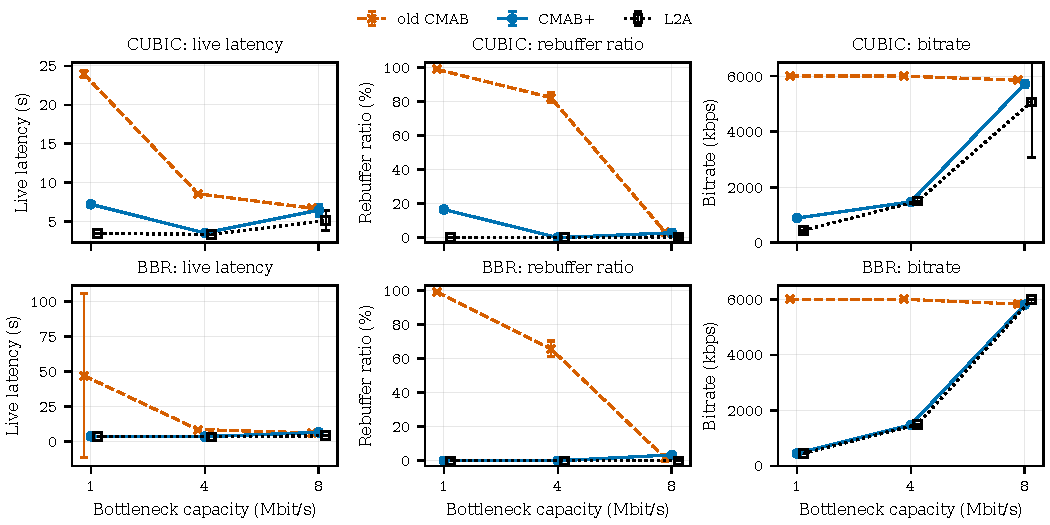
\includegraphics[width=\textwidth]{figures/capacity}
\Description{Grid of six panels: latency, rebuffer and bitrate against bottleneck capacity for old CMAB, CMAB+ and L2A-LL, under CUBIC and BBR.}
\caption{Capacity experiment at a 3\,s target: mean of 5 sessions with 95\% $t$ intervals, CUBIC (top) and BBR (bottom). At 4 and 1\,Mbit/s old CMAB stays on the 6000\kbps rung and rebuffers most of the time; CMAB+ follows the feasible rung. The wide BBR 1\,Mbit/s latency interval for old CMAB comes from one 131\,s session.}
\label{fig:capacity}
\end{figure*}

\begin{figure*}[t]
\centering
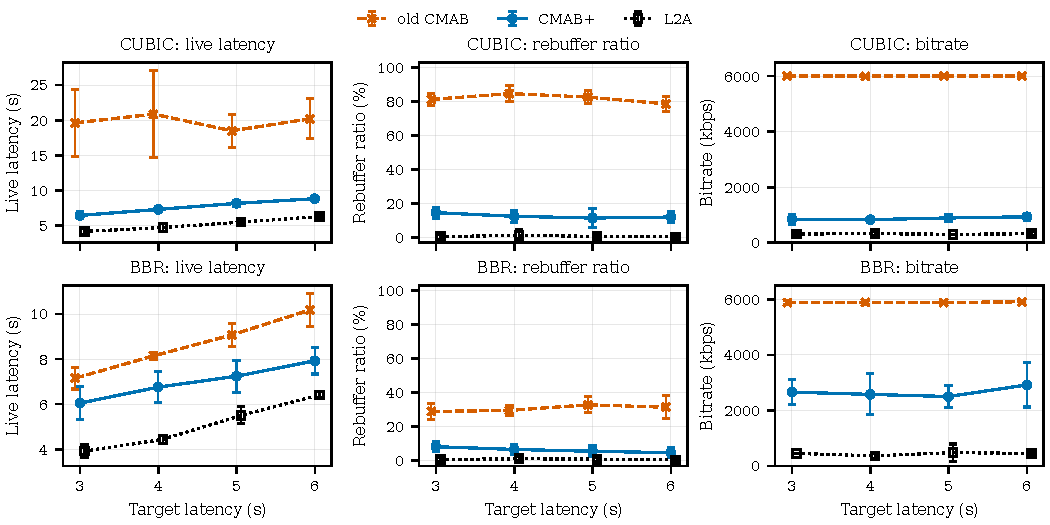
\includegraphics[width=\textwidth]{figures/trace}
\Description{Grid of six panels: latency, rebuffer and bitrate against latency target on the ISL trace for old CMAB, CMAB+ and L2A-LL, under CUBIC and BBR.}
\caption{Starlink ISL trace shaper, final CMAB+ player (rules 1--5): mean of 5 sessions with 95\% $t$ intervals, CUBIC (top) and BBR (bottom). CMAB+ leaves old CMAB's 6000\kbps lock and cuts rebuffering at every target, but L2A-LL keeps rebuffering near 1\% at a much lower bitrate.}
\label{fig:trace}
\end{figure*}

\paragraph{Pass criteria.} We fixed three gates before running the matrices. On the paper clock \cmabp must stay in the same class as \oldcmab: similar bitrate, near-zero rebuffering, latency within a few tenths of a second. At 4\,Mbit/s it must avoid collapse at every target. On the trace it must rebuffer less than \oldcmab without settling on the bottom rung as its only operating point.

\section{Evaluation}
\label{sec:eval}

\subsection{No regression on the paper clock}
\label{sec:nonreg}

Table~\ref{tab:nonreg} shows that \cmabp tracks \oldcmab on the paper's 100\,Mbit/s clock shaper under both transports. \cmabp is never more than 0.15\,s slower (CUBIC, 3\,s target, where the 95\% intervals of the two players overlap), and it is 0.28\,s faster under BBR at 5\,s. It plays 3 to 141\kbps more on average in seven of eight cells and 11\kbps less in the eighth. Rebuffering is zero in every CUBIC cell. Under BBR, \oldcmab rebuffers 0.26\% at 5\,s and \cmabp 0.08\% at 5\,s and 0.38\% at 6\,s; all three intervals include zero. L2A-LL plays 6000\kbps and is 0.15--0.38\,s closer to the target than \cmabp. On a link that carries every rung, \cmabp and \oldcmab end up in the same operating range.

These clock runs were measured with rules 1--4. The stall guard was added later. We ran spot batches of the final player at a 3\,s target on the clock and 4\,Mbit/s paths. The project ledger records both as unchanged, but those session trees are not in the archives, so we cannot report numbers for them, and we did not rerun the full matrices.

\begin{table}[t]
\caption{Non-regression on the paper clock (100\,Mbit/s; 50\,Mbit/s, 100\,ms, 1\% loss in handover seconds). Mean of 5 sessions: latency (s) / bitrate (kbps). Rebuffer is 0\% except under BBR: old CMAB 0.26\% at 5\,s, CMAB+ 0.08\% at 5\,s and 0.38\% at 6\,s.}
\label{tab:nonreg}
\footnotesize
\begin{tabular}{@{}llccc@{}}
\toprule
TCP & Target & old CMAB & CMAB+ & L2A-LL \\
\midrule
\multirow{4}{*}{CUBIC} & 3 s & 4.09 / 5363 & 4.24 / 5420 & 4.02 / 6000 \\
 & 4 s & 4.52 / 5292 & 4.54 / 5433 & 4.37 / 6000 \\
 & 5 s & 5.29 / 5430 & 5.24 / 5448 & 5.03 / 6000 \\
 & 6 s & 6.28 / 5378 & 6.27 / 5462 & 6.02 / 6000 \\
\midrule
\multirow{4}{*}{BBR} & 3 s & 3.45 / 5251 & 3.44 / 5255 & 3.06 / 6000 \\
 & 4 s & 4.21 / 5252 & 4.23 / 5290 & 4.08 / 6000 \\
 & 5 s & 5.51 / 5201 & 5.23 / 5285 & 5.08 / 6000 \\
 & 6 s & 6.23 / 5340 & 6.31 / 5329 & 6.06 / 6000 \\
\bottomrule
\end{tabular}
\end{table}

The CUBIC latencies here are about 0.9\,s higher than in Review~I at a 3\,s target (4.09\,s against 3.19\,s for \oldcmab), and L2A-LL on the same runs moved from 3.00 to 4.02\,s. Both players shifted, so the cause lies in the testbed between the September and November runs. We have not isolated it, and we compare players only within a batch.

\subsection{Capacity: where collapse appears}
\label{sec:capacity}

Figure~\ref{fig:capacity} and Table~\ref{tab:capacity} show the capacity experiment. At 4\,Mbit/s, \oldcmab requests 6000\kbps in every session and rebuffers 82.25\% of the time under CUBIC and 65.69\% under BBR, with about 8.6\,s of latency at a 3\,s target. \cmabp selects the 1500\kbps rung almost all the time (1473 and 1477\kbps on average), has no rebuffering, and reaches 3.54 and 3.62\,s, a 58--59\% latency reduction. L2A-LL on the same runs picks 1500\kbps at 3.36 and 3.40\,s, so \cmabp is 0.18--0.22\,s behind it.

At 1\,Mbit/s the outcome depends on the transport. Under BBR, \cmabp matches L2A-LL at 450\kbps with no rebuffering. Under CUBIC it plays mostly the 900\kbps rung (mean 888\kbps), which fits $\That$ but not the sustained rate, and rebuffers 16.54\%; L2A-LL stays at 450\kbps with none. Rules 1 and 2 allow any rung at or below $\That$, with no spare margin, and this cell shows the cost. The BBR \oldcmab mean of 47.04\,s includes one 131.26\,s session; the other four are 25.61--26.37\,s and all five rebuffer 98.7--100\%.

At 8\,Mbit/s the top rung nominally fits (8\,Mbit/s is 1.33 times 6000\kbps), and \cmabp does not improve on \oldcmab. Both run at 6.2--6.7\,s with 1.8--3.5\% rebuffering, and L2A-LL is better under both transports.



\begin{table}[t]
\caption{Capacity experiment, 3\,s target, mean of 5 sessions: latency (s) / rebuffer (\%) / bitrate (kbps).}
\label{tab:capacity}
\footnotesize
\setlength{\tabcolsep}{3pt}
\begin{tabular}{@{}llccc@{}}
\toprule
TCP & Cap. & old CMAB & CMAB+ & L2A-LL \\
\midrule
\multirow{3}{*}{CUBIC} & 8 & 6.73 / 3.31 / 5854 & 6.48 / 2.85 / 5721 & 5.15 / 0.45 / 5075 \\
 & 4 & 8.58 / 82.25 / 6000 & 3.54 / 0 / 1473 & 3.36 / 0 / 1500 \\
 & 1 & 23.96 / 98.79 / 6000 & 7.23 / 16.54 / 888 & 3.47 / 0 / 450 \\
\midrule
\multirow{3}{*}{BBR} & 8 & 6.22 / 1.77 / 5828 & 6.63 / 3.49 / 5804 & 4.32 / 0 / 6000 \\
 & 4 & 8.66 / 65.69 / 6000 & 3.62 / 0 / 1477 & 3.40 / 0 / 1500 \\
 & 1 & 47.04 / 99.13 / 6000 & 3.85 / 0 / 450 & 3.69 / 0 / 450 \\
\bottomrule
\end{tabular}
\end{table}

\subsection{\texorpdfstring{4\,Mbit/s}{4 Mbit/s} at every target}
\label{sec:robust}

The capacity result holds at every target (Table~\ref{tab:robust}). Old CMAB stays at 6000\kbps and rebuffers 71.70--80.59\% under CUBIC and 62.05--69.23\% under BBR, with latency 5.6--5.9\,s above the target. \cmabp has no rebuffering in any of its 40 sessions and plays 1457--1477\kbps. It lands 0.20--0.23\,s above the 4, 5 and 6\,s targets and 0.54--0.62\,s above the 3\,s target; its latency is 46.5--58.7\% lower than \oldcmab's. L2A-LL sits on the target at 4--6\,s and at 3.35--3.41\,s for a 3\,s target, so \cmabp trails it by 0.19--0.23\,s in every cell. The 95\% intervals of \cmabp latency are at most $\pm$0.05\,s, so that gap is consistent across sessions.

\begin{table}[t]
\caption{4\,Mbit/s clock at targets 3--6\,s, mean of 5 sessions. Old CMAB: latency (s) / rebuffer (\%), always 6000\kbps. CMAB+ and L2A-LL: latency (s) / bitrate (kbps), 0\% rebuffer in every cell.}
\label{tab:robust}
\footnotesize
\begin{tabular}{@{}llccc@{}}
\toprule
TCP & Target & old CMAB & CMAB+ & L2A-LL \\
\midrule
\multirow{4}{*}{CUBIC} & 3 s & 8.56 / 80.59 & 3.54 / 1457 & 3.35 / 1500 \\
 & 4 s & 9.62 / 78.83 & 4.20 / 1467 & 4.00 / 1500 \\
 & 5 s & 10.59 / 78.90 & 5.21 / 1472 & 5.00 / 1500 \\
 & 6 s & 11.64 / 71.70 & 6.23 / 1469 & 6.00 / 1500 \\
\midrule
\multirow{4}{*}{BBR} & 3 s & 8.62 / 62.05 & 3.62 / 1474 & 3.41 / 1500 \\
 & 4 s & 9.59 / 64.01 & 4.21 / 1477 & 4.00 / 1500 \\
 & 5 s & 10.86 / 65.40 & 5.22 / 1472 & 5.00 / 1500 \\
 & 6 s & 11.85 / 69.23 & 6.23 / 1475 & 6.00 / 1500 \\
\bottomrule
\end{tabular}
\end{table}

\subsection{Starlink ISL trace with the stall guard}
\label{sec:trace}

The trace is the hardest case (Figure~\ref{fig:trace}, Table~\ref{tab:trace}). Old CMAB collapses under both transports: under CUBIC it plays 6000\kbps and rebuffers 78.55--84.61\% with 18.5--20.9\,s of latency; under BBR it plays about 5900\kbps and rebuffers 28.98--32.88\%. With all five rules, \cmabp leaves the top rung. At a 3\,s target its rebuffering falls from 81.14\% to 14.67\% under CUBIC (at 851\kbps) and from 28.98\% to 8.29\% under BBR (at 2658\kbps). Across all eight cells the reduction is 71.4--86.0\%, and latency falls by 1.1--13.5\,s.

Before the stall guard, the same matrix gave \cmabp 30.84--35.22\% rebuffering under CUBIC at 1578--1776\kbps, and 8.92--11.71\% under BBR (\path{report/results/trace-pre-stallguard-aggregate.csv}). The guard brings CUBIC down to 11.52--14.67\% and BBR to 4.75--8.29\%, and costs bitrate in both. It does this by holding a low rung after an empty buffer until 12 healthy decisions have passed, which is slower to recover than rule~3 alone.

\cmabp does not reach L2A-LL here. L2A-LL rebuffers 0.49--1.43\% at 301--482\kbps, with latency 2.3--2.7\,s lower than \cmabp under CUBIC and 1.5--2.3\,s lower under BBR. \cmabp plays 2.5 to 3 times L2A-LL's bitrate under CUBIC and 5 to 7 times under BBR, for 4--14 percentage points more rebuffering. Whether that trade is worth making depends on the service; where rebuffering dominates the cost, L2A-LL's choice is safer.


\begin{table}[t]
\caption{ISL trace at targets 3--6\,s, mean of 5 sessions: latency (s) / rebuffer (\%) / bitrate (kbps).}
\label{tab:trace}
\footnotesize
\setlength{\tabcolsep}{2.6pt}
\begin{tabular}{@{}llccc@{}}
\toprule
TCP & Tgt. & old CMAB & CMAB+ & L2A-LL \\
\midrule
\multirow{4}{*}{CUBIC} & 3 & 19.62 / 81.14 / 6000 & 6.46 / 14.67 / 851 & 4.19 / 0.52 / 316 \\
 & 4 & 20.87 / 84.61 / 6000 & 7.32 / 12.53 / 832 & 4.75 / 1.43 / 329 \\
 & 5 & 18.50 / 82.52 / 6000 & 8.18 / 11.52 / 893 & 5.52 / 0.69 / 301 \\
 & 6 & 20.20 / 78.55 / 6000 & 8.84 / 12.09 / 935 & 6.30 / 0.49 / 330 \\
\midrule
\multirow{4}{*}{BBR} & 3 & 7.16 / 28.98 / 5882 & 6.05 / 8.29 / 2658 & 3.91 / 0.77 / 449 \\
 & 4 & 8.14 / 29.60 / 5887 & 6.76 / 6.67 / 2575 & 4.44 / 1.21 / 360 \\
 & 5 & 9.07 / 32.88 / 5884 & 7.24 / 5.60 / 2499 & 5.50 / 0.93 / 482 \\
 & 6 & 10.19 / 31.45 / 5913 & 7.93 / 4.75 / 2917 & 6.41 / 0.51 / 444 \\
\bottomrule
\end{tabular}
\end{table}

\subsection{Comparison with L2A-LL}
\label{sec:l2a}

Across the four experiments, \cmabp is close to L2A-LL in two places: at 4\,Mbit/s (0.18--0.23\,s behind, same rung, no rebuffering) and at 1\,Mbit/s under BBR. L2A-LL has lower latency and rebuffering at 8\,Mbit/s, at 1\,Mbit/s under CUBIC and on the trace, and lower latency with higher bitrate on the paper clock. \cmabp plays a higher bitrate than L2A-LL on the trace and at 8 and 1\,Mbit/s under CUBIC, each time with more rebuffering. Our supported claim is narrow. When the forced window asks for a rung the link cannot carry, \cmabp keeps playback going; at 4\,Mbit/s it also brings latency to within 0.62\,s of the target. On links that carry the top rung it behaves like \oldcmab.

\section{Discussion and limitations}
\label{sec:discussion}

\paragraph{Why the bug survived.} The artifact's emulator runs at 100\,Mbit/s with 50\,Mbit/s during handovers, far above the 6000\kbps top rung. A forced top-rung window costs nothing there, so the emulation results could not expose it. The paper's dish runs used a terminal without ISLs; we cannot say how often a real dish falls below 6\,Mbit/s for a full slot. Our capacity shaper forces that condition on purpose.

\paragraph{What we did not measure.} We had no dish, so we cannot claim results on a live Starlink link. The trace shaper replays one hour of RTT samples from one installation, with handover loss modeled as 100\% for the zero-RTT rows; real handovers vary by location, time and load. Each Review~III cell has five rounds; the \cmabp intervals are tight at 4\,Mbit/s and wide for some trace and 1\,Mbit/s cells, and ten rounds per cell would narrow them. The paper-clock and 4\,Mbit/s multi-target matrices used rules 1--4; the stall guard was checked there only by spot runs. We reran neither Dynamic nor LoL+ in Review~III. Our rebuffer metric counts buffer samples at the floor and does not equal the paper's rebuffering-time ratio, which also limits the comparison with the paper's Figure~8.

\paragraph{Open problems.} Rules 1 and 2 accept any rung at or below $\That$; the 1\,Mbit/s CUBIC cell shows that this is too aggressive when the estimate is noisy, and a margin or a variance-aware cap may help. The artifact passes P.1203 an empty stalling list, so stalls reach the reward only through the bounded share-of-rebuffering term, and the bandit learns little from them; changing that would change the learner, which we left alone. The latency gap to the paper's 3\,s result in Review~I is also unexplained.

\section{Related work}
\label{sec:related}

\paragraph{Starlink measurement.} Michel et al.~\cite{michel2022firstlook} gave an early view of Starlink throughput and latency, and Mohan et al.~\cite{mohan2024multifaceted} combined crowdsourced and controlled measurements across regions. Zhao et al.~\cite{zhao2023reality} studied video-on-demand, live streaming and conferencing over Starlink and found that large VoD buffers absorb handovers while interactive services suffer. Tanveer et al.~\cite{tanveer2023constellations} identified the 15\,s global schedule, and Pan et al.~\cite{pan2023measuring} mapped the access, gateway and backbone architecture. These works motivate a slot-aware controller; none of them proposes one.

\paragraph{Low-latency ABR.} Dynamic~\cite{spiteri2019dynamic} and BOLA~\cite{spiteri2020bola} are the default dash.js logic. L2A-LL~\cite{karagkioules2020l2a} frames bitrate choice as online convex optimization and needs no throughput model. LoL+~\cite{bentaleb2022lolp} adds a learned weight selection and playback-speed control. O'Hanlon and Aslam~\cite{ohanlon2023latency} compared the three across latency targets on terrestrial traces. Zhao and Pan~\cite{zhao2024mmsys} added the LinTS controller we study. \cmabp is closer in spirit to the throughput rule in Dynamic than to a new learner: it bounds what the bandit may request by what the network has delivered.

\paragraph{Transport over Starlink.} The MMSys '24 paper notes that Starlink TCP throughput suffers from repeated slow starts at handovers and suggests BBR or satellite-aware control such as SaTCP~\cite{cao2023satcp}. Under our clock shaper, swapping CUBIC for BBR moved CMAB latency by 0.1\,s at a 3\,s target; under the capacity and trace shapers BBR helped \oldcmab (65.69\% against 82.25\% rebuffering at 4\,Mbit/s) without removing the collapse. In this setup the ABR's request policy mattered more than the congestion controller.

\section{Conclusion}

We reproduced the MMSys '24 emulation, ran it again under BBR, and found that the first BBR failure came from a shaper misconfiguration. Following that failure into the code exposed a forced window that requests the top rung after every Starlink slot boundary. Five rules around the unchanged LinTS learner stop the resulting collapse: at 4\,Mbit/s, rebuffering drops from 62--82\% to zero at every target, and on the paper's own shaper the player behaves like \oldcmab. On the trace shaper the rules cut rebuffering by 71--86\% but do not reach L2A-LL. The next steps are a dish measurement, ten-round matrices with the final player on every shaper, and a stall signal the bandit can learn from.

\begin{acks}
We thank the CS G525 course at BITS Pilani for feedback at each review, and Dr.~Yash Sinha for his guidance as course tutor.
\end{acks}

%%% END BODY
\label{body:end}

\balance
\bibliographystyle{ACM-Reference-Format}
\bibliography{reference}

\appendix

\section{Artifact}
\label{app:artifact}

\paragraph{Code.} The modified artifact is at \url{https://github.com/pratham-commits/CMAB_plus} (branch \texttt{main}, commit \texttt{d60f163})~\cite{cmabplus}, forked from the authors' repository at \texttt{dc120de}. The \cmabp rules are in \path{dash.js/src/streaming/rules/abr/cmab/cmabPlusPolicy.js} and are wired into \path{CMABAbrController.js}; \path{experiments/test_cmab_plus_policy.mjs} unit-tests them without Docker. Each matrix has a batch file (\path{experiments/batch-*.json}) and a runner script (\path{experiments/run-*.sh}); the capacity runners check the congestion control and the \texttt{tc} qdisc and rate inside the nginx container before every batch. The course repository holds the review packages and analysis scripts (\path{review-3/analyze_*.py}); each script rebuilds its results table, CSVs and figures from the extracted session data and stops if the session count is not the expected one.

\paragraph{Data.} Table~\ref{tab:archives} lists the Review~III archives with their SHA-256 digests, which we re-checked against \path{review-3/DATA_MANIFEST.md} before writing this report. The Review~II BBR clock dataset (prefix \texttt{1017-0606}) and the superseded trace run (prefix \texttt{1010-0432}) are under \path{review-ii-bbr-extension/}.

\begin{table*}[t]
\caption{Review III data archives (\texttt{review-3/data/archives/}).}
\label{tab:archives}
\footnotesize
\begin{tabular}{@{}lrl@{}}
\toprule
Archive & Sessions & SHA-256 \\
\midrule
\texttt{cmab-plus-clock-nonreg-cubic.tar.gz} & 60 & \texttt{55716f33b860b4ba1f2c6b0fe4d3c8d3fdaa532d989062707c06ef7d9806f8f3} \\
\texttt{cmab-plus-clock-nonreg-bbr.tar.gz} & 60 & \texttt{1b29c2ac41bde0f3c9b32fe817ee80d49acc3ef240c7fda9d021658fa7e41f5f} \\
\texttt{cmab-plus-capacity-cubic.tar.gz} & 45 & \texttt{0040b3d46a0b202ce0f734e383ef57e4876bb580b5874426df905c627050b14f} \\
\texttt{cmab-plus-capacity-bbr.tar.gz} & 45 & \texttt{c62c01d2bdf15222ebdb5318393d59b7ebb93cb2c671e93f64dd4e5c409d9e9d} \\
\texttt{cmab-plus-capacity-4mbit-targets-cubic.tar.gz} & 60 & \texttt{21b29deccba1f3f202351ce10b85184162ca8a46fd8afea1d664afcef3d1cef0} \\
\texttt{cmab-plus-capacity-4mbit-targets-bbr.tar.gz} & 60 & \texttt{0141ed96b2a282199a9824587c654c197fc496cc86005ed3de3ff8c77146bde7} \\
\texttt{cmab-plus-trace-stallguard-cubic-bbr-20261108.tar.gz} & 120 & \texttt{27cdf2a5493e126a84390ac889dbc77933aab0f01ad96d4673e8adda97c20d0a} \\
\texttt{cmab-plus-cubic-1102-1304.tar.gz} (trial 7) & 160 & \texttt{0652cda3862b6759a8bbd300ced771d9ec87c7461828a36a90bdc2319a561028} \\
\bottomrule
\end{tabular}
\end{table*}

\paragraph{Report sources.} This report lives in \path{report/}. \path{report/scripts/pre_stallguard_trace.py} aggregates the pre-stall-guard trace trees kept under \path{review-3/data/}. \path{report/scripts/review12_tables.py} recomputes Table~\ref{tab:review12} and Table~\ref{tab:review12full} from the Review~I and II session trees, and \path{report/scripts/make_figures.py} draws every figure from the committed aggregate CSVs and, for Figure~\ref{fig:timeline}, from two raw 4\,Mbit/s sessions.

\paragraph{Demo.} \path{review-3/demo-ui} is a browser replay of logged sessions. It plays three panes side by side (for example \oldcmab, \cmabp and L2A-LL), drives each pane's bitrate and stalls from the recorded timelines, marks the 15\,s handover clock, and includes pages for the algorithm and for the problems we hit in each review.

\section{Full Review I and II results}
\label{app:review12}

Table~\ref{tab:review12full} gives every target for the three datasets. Rebuffering is 0.00\% in all D1 and D3 cells except D1 CMAB at 5\,s (2.52\%, from the single outlier round in Section~\ref{sec:repro}) and D3 LoL+ at 3\,s (0.01\%).

\begin{table*}[t]
\caption{Review I (D1) and Review II (D3, D2) at all targets: mean of 10 sessions. D1 and D3 cells are latency (s) / bitrate (kbps); D2 cells are latency (s) / rebuffer (\%) / bitrate (kbps).}
\label{tab:review12full}
\footnotesize
\begin{tabular}{@{}lcccccccc@{}}
\toprule
 & \multicolumn{4}{c}{D1: CUBIC, clock} & \multicolumn{4}{c}{D3: BBR, clock} \\
\cmidrule(lr){2-5}\cmidrule(l){6-9}
ABR & 3 s & 4 s & 5 s & 6 s & 3 s & 4 s & 5 s & 6 s \\
\midrule
Dynamic & 3.00 / 5909 & 4.00 / 5910 & 5.00 / 5640 & 6.01 / 5600 & 3.12 / 5123 & 4.01 / 5679 & 5.00 / 5824 & 6.00 / 5744 \\
L2A-LL  & 3.00 / 6000 & 4.02 / 6000 & 5.00 / 6000 & 6.02 / 6000 & 3.11 / 6000 & 4.01 / 6000 & 5.00 / 6000 & 6.00 / 6000 \\
LoL+    & 3.08 / 4938 & 4.07 / 4902 & 5.08 / 4900 & 6.11 / 4900 & 3.14 / 5454 & 4.08 / 4974 & 5.09 / 4906 & 6.11 / 4900 \\
CMAB    & 3.19 / 4955 & 4.20 / 4989 & 6.05 / 4951 & 6.24 / 5021 & 3.29 / 5223 & 4.21 / 5167 & 5.21 / 5165 & 6.23 / 5205 \\
\midrule
 & \multicolumn{8}{c}{D2: BBR, trace (superseded first run)} \\
\cmidrule(l){2-9}
ABR & \multicolumn{2}{c}{3 s} & \multicolumn{2}{c}{4 s} & \multicolumn{2}{c}{5 s} & \multicolumn{2}{c}{6 s} \\
\midrule
Dynamic & \multicolumn{2}{c}{4.13 / 1.10 / 619} & \multicolumn{2}{c}{4.68 / 0.58 / 881} & \multicolumn{2}{c}{5.58 / 0.22 / 1044} & \multicolumn{2}{c}{6.36 / 0.28 / 1350} \\
L2A-LL  & \multicolumn{2}{c}{3.81 / 0.59 / 359} & \multicolumn{2}{c}{4.57 / 1.10 / 436} & \multicolumn{2}{c}{5.40 / 0.93 / 421} & \multicolumn{2}{c}{6.40 / 0.82 / 421} \\
LoL+    & \multicolumn{2}{c}{4.64 / 5.40 / 861} & \multicolumn{2}{c}{5.33 / 4.72 / 1067} & \multicolumn{2}{c}{6.88 / 6.99 / 2146} & \multicolumn{2}{c}{7.50 / 6.81 / 1930} \\
CMAB    & \multicolumn{2}{c}{7.19 / 28.32 / 5795} & \multicolumn{2}{c}{8.13 / 31.16 / 5819} & \multicolumn{2}{c}{9.08 / 29.85 / 5870} & \multicolumn{2}{c}{9.84 / 27.84 / 5834} \\
\bottomrule
\end{tabular}
\end{table*}

\end{document}
